% siminos/dimension/ver0/DCTSCD14.tex   pdf DCTSCD14
% $Author: predrag $ $Date: 2016-02-03 23:17:20 -0500 (Wed, 03 Feb 2016) $

%% logical setup, no need to edit %%%%%%%%%%
\newif\ifboyscout                         %%
\boyscoutfalse %% commented, WWW/boyscouts %%
\newif\ifpreparepdf                       %%
\preparepdftrue % hyperlinked pdf default %%

                        % Toggle between draft and non-draft versions
% \boyscoutfalse                 % public, hyperlinked
% \preparepdffalse               % for B&W, print version

%                    PRL resubmission: Xiong    ??? 12 2015
%                    arXiv submission: Xiong    ??? 12 2015
%                    finished editing: Predrag  ??? 11 2015
% Note: {revtex4} has been replaced by {revtex4-1} by APS
%       revert to {revtex4} if you have an old configuration
%       read also sliceDefs.tex
%                    finished rewriting: Xiong  ??? ?? 2015
%                    PRL rejection:             ??? ?? 2015
%                    PRL submission:   Xiong    ??? 2? 2015
%                    arXiv submission: Xiong    ??? 24 2015
%                    Predrag completed rewrite  ??? 30 2015
%                    Xiong 1. draft slice.tex   ???  9 2015
%                    Xiong created the template May  9 2015


%% ------------------ for arXiv-v1 submission ----------------------------
%
% Title:    TITLE?
% Authors:  Xiong Ding, Predrag Cvitanovi\'c,
%           Ruslan L. Davidchack, and Evangelos Siminos
%
% Comments: 4 pages, 4 pdf and 6 png figures, uses revtex4
% Files:    slice.tex sliceDefs.tex slice.bbl
%           dim-2mode1.pdf dim-2mode2.pdf
%           dim-kssspfull.pdf dim-kssspred.pdf
%  dim-ksconftw.png dim-ksconftwred.png dim-ksconftwredtau.png
%  dim-ksconfrpo.png dim-ksconfrpored.png dim-ksconfrporedtau.png
%
%% ------------------ cut here ----------------------------------------



\ifboyscout
\documentclass[prl,aps,preprint,showpacs]{revtex4-1} %or {revtex4}
\else
\documentclass[prl,aps,twocolumn,showpacs,superscriptaddress]{revtex4-1} %or {revtex4}
\fi
% \documentclass[aps,pre, reprint,groupedaddress]{revtex4-1}
\usepackage[dvipdfmx]{graphicx}


\input defsDim

\bibliographystyle{apsrev4-1}  %or {apsrev4}

\graphicspath{ {../../xiong/figures/} }

\begin{document}

\title{The lower bound of physical dimension
  of 1D Kuramoto-Sivashinsky system}

\author{X. Ding}
\author{P. Cvitanovi\'c}
\affiliation{
                Center for Nonlinear Science, School of Physics,
                Georgia Institute of Technology,
                Atlanta, GA 30332-0430
               }
\author{K. A. Takeuchi}
\author{H. Chat\'e}
\author{E. Siminos}
\author{R. L. Davidchack}


\date{\today}

\begin{abstract}
  We study the partial hyperbolicity of periodic orbits in
  dissipative chaotic systems via the associated Floquet vectors in
  the tangent space. And, by projecting Floquet vectors onto the
  symmetry reduced state space, we investigate shadowing events
  between ergodic and periodic orbits and find the effective
  expansion of difference vector. These two numerical experiments explain the
  topological structure of the tangent bundle along periodic orbits
  and give a lower bound on the dimension of inertial manifold
  of 1D Kuramoto-Sivashinsky system.
\end{abstract}


\pacs{}
%\keywords{}

\maketitle


Dynamics in dissipative systems usually land on an
\inm\rf{temam90, Foias1988a, Robinson1995}
after a
transient period of evolution. This forward in time exponentially attracting
invariant manifold contains the global attractor and
simplifies the study of the asymptotic dynamics since it is finite
dimensional. The existence of \inm\ has been proved for several
systems, such as \KSe, \cGLe, and reaction-diffusion equations\rf{infdymnon}.
On one hand, mathematicians are continuing to improve the
upper bounds on the dimension of \inm\ for some dynamical systems
(see \refrefs{CEEksgl93,jolly_evaluating_2000,Robinson-PLA1994}
for a series of results for one dimensional
\KSe);
at the same time,  numerical experiments conducted on
\cLv s\rf{GiChLiPo12, YaTaGiChRa08}
demonstrate that the tangent bundle of ergodic trajectories
is decomposed into two dynamically decoupled invariant sub-bundles, one
of which is strictly contracting and the other contains the whole
set of expanding directions and a subset of contracting directions. The
numerical results suggests that the dimension of \inm\
should be larger than Kaplan-Yorke dimension but much smaller than the
mathematical upper bound.

On the other hand,
as shown by P. Cvitanovi\'c and coworkers\rf{DasBuch},
the effective dynamics in chaotic
systems can be visualized as a walk chaperoned
by a hierarchy of unstable invariant solutions (equilibria, periodic orbits
and invariant tori) embedded in the attractor. Moreover,
if the symbolic dynamics coding this walk is known, then asymptotic
properties is totally determined by a subset of short periodic orbits.
From this geometrical
point of view, \Fv s associated with \po s should suffice to give
information about the dimension of \inm\ as \cLv s along ergodic
trajectories do, and this is the main purpose of this article.

In this letter, we study the geometrical and dynamical properties of
\Fv s to give a lower bound on the dimension of \inm. More specially,
we study the partial hyperbolicity\rf{Pesin2004}
of periodic orbits by the concept
of local \Fe\ and measure the angle distribution of
subspaces formed by \Fv s as did by predecessors with
\cLv s. Also, inspired by the study of projection of difference
vector onto subspace spanned by \cLv s\rf{YaRa11},
we study the shadowing events
between ergodic trajectories and periodic orbits. Note, our
numerical experiments
are novel because we take advantage of invariant set not ergodic
trajectories, and an efficient algorithm\rf{DingCvit14} for computing
\Fv s. More importantly, we reduce the continuous symmetry
of the system when hunting for shadowing events and project \Fv s
into this symmetry reduced state space.

Throughout this letter, we focus on 1D \KSe\rf{kuramoto1975, michsiv77}
\begin{equation}
  u_t+\frac{1}{2}(u^2)_x+u_{xx}+u_{xxxx}=0\,,\; x\in [0,L]
  \label{eq:ks}
\end{equation}
on a periodic domain of size $L=22$, large enough to
exhibit complex spatiotemporal chaotic dynamics\rf{SCD07}.
This system is
invariant under Galilean transformation $u(x,t)\to u(x-ct, t)+c$,
reflection $u(x,t)\to -u(-x,t)$ and spatial translation
$u(x,t) \to u(x+\ell,t)$.
The Galilean invariance is
enforced in the integrator; Consequently, we have two different
types of invariant orbit: pre-\po\  $u(x, 0) = Ru(x,T_p)$
and relative \po\ $u(x, 0) = g(\theta_p)u(x, T_p)$.
Here, $R$ is a reflection operation and $g(\theta_p)$ is the
spatial translation by amount $\frac{L}{2\pi}\theta_p$.
Our experiments are conducted with 200 pre-\po s\ and 200 relative
\po s, and make no distinction between them when doing statistics.

% \begin{figure}[h]
%   \centering
%   \begin{minipage}{.1\textwidth}
%     \centering \small{\texttt{(a)}}
%     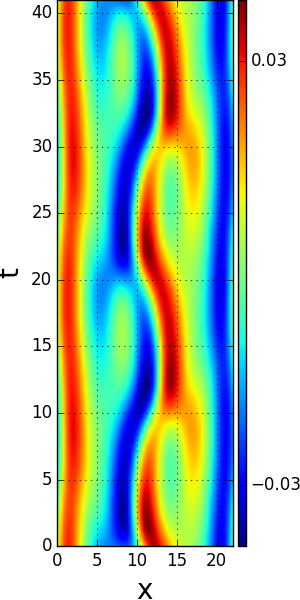
\includegraphics[width=\textwidth]{ppo1State64}
%   \end{minipage}
%   \begin{minipage}{.08\textwidth}
%     \centering \small{\texttt{(b)}}
%     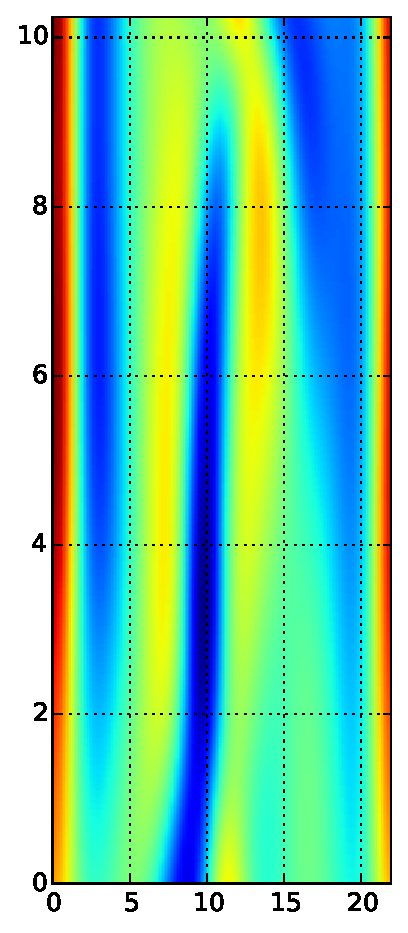
\includegraphics[width=\textwidth]{ppo1Fv1_64}
%   \end{minipage}
%   \begin{minipage}{.08\textwidth}
%     \centering \small{\texttt{(c)}}
%     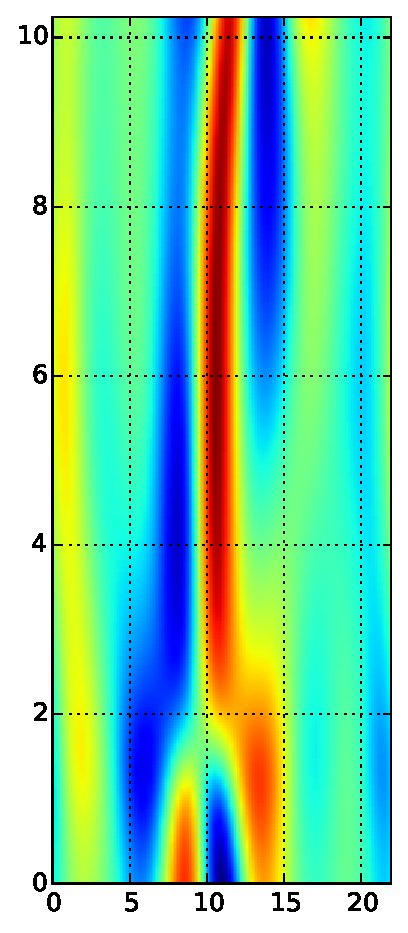
\includegraphics[width=\textwidth]{ppo1Fv5_64}
%   \end{minipage}
%   \begin{minipage}{.08\textwidth}
%     \centering \small{\texttt{(d)}}
%     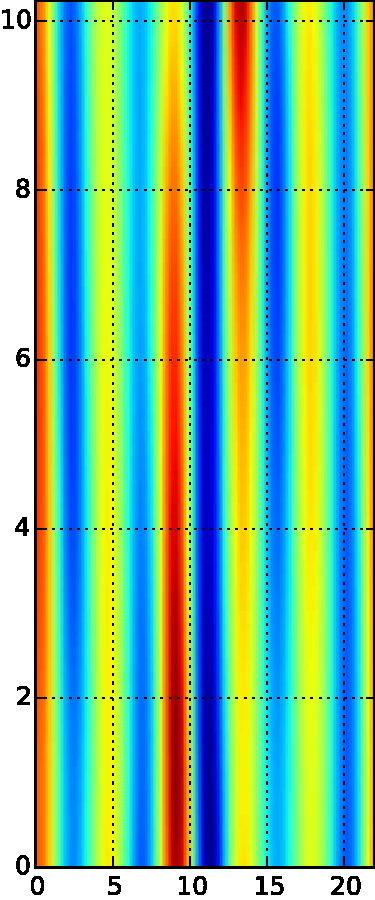
\includegraphics[width=\textwidth]{ppo1Fv10_64}
%   \end{minipage}
%   \begin{minipage}{.08\textwidth}
%     \centering \small{\texttt{(d)}}
%     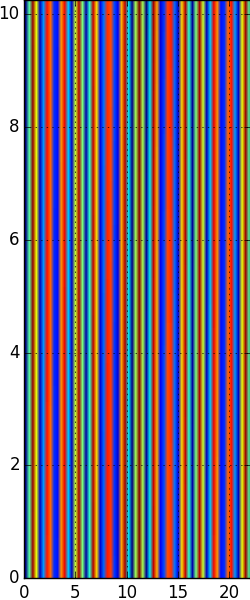
\includegraphics[width=\textwidth]{ppo1Fv30_64}
%   \end{minipage}
%   \caption{(Color on line)
%   }
%   \label{fig:ppo1}
% \end{figure}

Let $\op = f^t(\op_0)$ be an orbit of an autonomous flow field
$\dot{\op} = v(\op)$. Linear proximately, infinitesimal
perturbation $\delta \op_0$ at point $\op_0$ is transported down the
orbit by the Jacobian of this orbit:
$J^t(\op_0) = \partial f^t(\op) / \partial \op |_{\op_0}$.
For a periodic orbit $\op(0) = \op (T_p)$, the
eigenvalues and eigenvectors of $J^{T_p}(\op_0)$ characterize the
linear stability of the tangent bundle along this \po, which
are named \Fm s $\Lambda_k$ and \Fv s $\jEigvec[k](\op)$ respectively.
$\lambda_k = \ln|\Lambda_k|/T_p$ is called the \Fe.
Most orbits in our database have one or two expanding
directions and are not hyperbolic. Instead, we investigate
partial hyperbolicity of \po s, which states that one subset of
\Fv s has a uniform larger expanding rate compared with the the
remaining set. To be specific, define the local \Fe\ as
\begin{equation}
  \label{eq:1}
  \lambda_k(\op) = \lim_{\Delta t \to 0}
  \frac{1}{\Delta t}
  \ln
  \frac{||J^{\Delta t}(\op)\jEigvec[k](\op)||}
  {||\jEigvec[k](\op)||}
\end{equation}
and decompose the tangent space at $x$ as $T_xM=E \bigoplus F$. Then
$\min_{\jEigvec[k]\in E} \lambda_k(x,t)
 > \mu > \nu > \max_{\jEigvec[k]\in F} \lambda_k(x,t)$ for some
specific $\mu$ and $\nu$ and for all points $x$ on the orbit.
\refFig{fig:fe}
shows the \Fe s, local \Fe s, and the difference between these two
along pre-\po\ $\cycle{ppo}_{10.25}$
( we use \cycle{rpo} to represent relative \po,
\cycle{ppo} for pre-\po, and subscript indicates the period).
We can see that local \Fe\ of
the first 8 \Fv s are entangled and decoupled from the remaining
set, meaning these two subsets are partial hyperbolic.
We call this number the threshold of partial hyperbolicity (TPH).
Also, as shown
in panel (c) and (d), the shapes of the local \Fe s along
$\cycle{pp}_{10.25}$ are similar and have relative small oscillations
for \Fv s with index larger than 8. Such homogeneous property suggests
that the dynamics in these direction is uniformly
simple and complex dynamics
exists in the subspace spanned by the first 8 \Fv s.
\begin{figure}[h]
  \centering
  \begin{minipage}{.23\textwidth}
    \centering \small{\texttt{(a)}}
    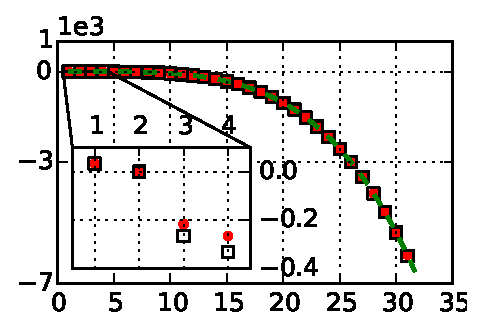
\includegraphics[width=\textwidth]{ppo1FEs}
  \end{minipage}
  \begin{minipage}{.23\textwidth}
    \centering \small{\texttt{(b)}}
    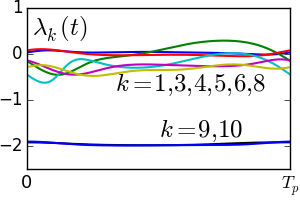
\includegraphics[width=\textwidth]{localFE1}
  \end{minipage}
  \begin{minipage}{.23\textwidth}
    \centering \small{\texttt{(c)}}
    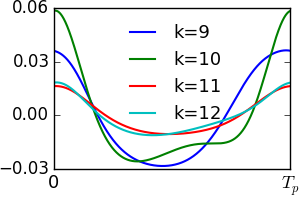
\includegraphics[width=\textwidth]{localFE2}
  \end{minipage}
  \begin{minipage}{.23\textwidth}
    \centering \small{\texttt{(d)}}
    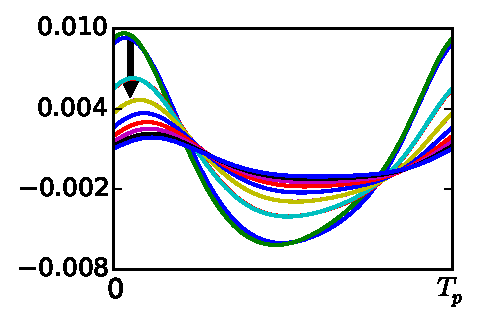
\includegraphics[width=\textwidth]{localFE3}
  \end{minipage}
  \caption{(Color online) (a) The \Fe s of $\cycle{pp}_{10.25}$ plotted
    pair wisely due to the degeneracy for high indices. Green line
    is $q_k^2-q_k^4$. (b) the leading 10 local \Fe s along.
    $\cycle{pp}_{10.25}$. \Fv s of $k = 1, 2$ and $k=6, 7$
    are complex conjugate pairs.
    (c) (d) $\lambda_k(\op) - \lambda_k$.
    In (d), $k$ goes from 13 to 27 as the black arrow indicates.
  }
  \label{fig:fe}
\end{figure}

Such partial hyperbolicity exists for all the orbits we have, and
\tph\ could be 8, 10, 12, 14, ... and so. Note, only even \tph s
are allowed because there is a degeneracy of 2 for \Fe s with
higher indices as shown in panel (a) of \reffig{fig:fe}.
However,  as suggested in panel (a) of
\reffig{fig:angle}, the minimum \tph\
is uniform for all \po s, which suggests that the global attractor
is partial hyperbolic with \tph\ 8. We believe this uniform
minimal \tph\ gives a lower bound on the dimension of \inm.
\begin{figure}[h]
  \centering
  \begin{minipage}{.18\textwidth}
    \centering \small{\texttt{(a)}}
    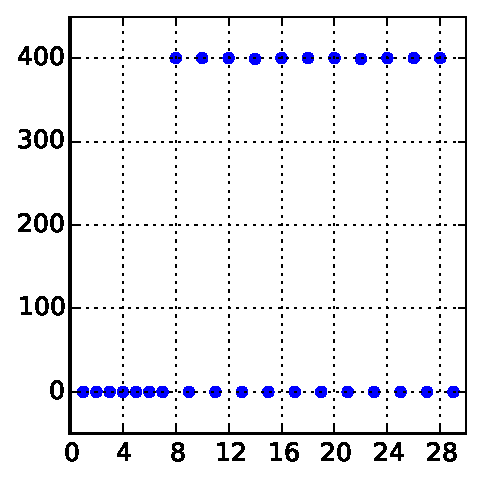
\includegraphics[width=\textwidth]{partialHyperb1}
  \end{minipage}
  \begin{minipage}{.28\textwidth}
    \begin{minipage}{\textwidth}
      \centering \small{\texttt{(b)}}
      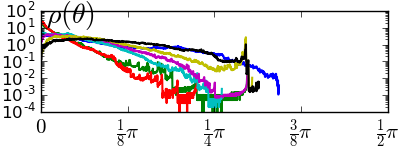
\includegraphics[width=\textwidth]{tangency1}
    \end{minipage}
    \begin{minipage}{\textwidth}
      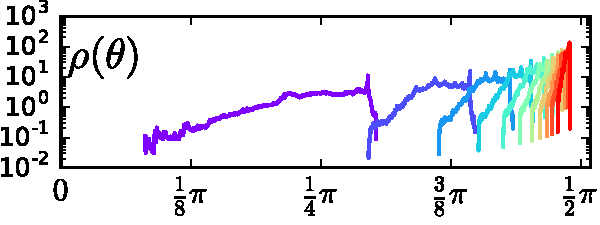
\includegraphics[width=\textwidth]{tangency2}
    \end{minipage}
  \end{minipage}
  \caption{(Color online)
    Total 400 \po s are used in the statistics.
    (a) the number of partial hyperbolic \po s versus different
    \tph s of
    (b) probability distribution of
    the minimal principal angle\rf{Knyazev02} between
    the two subspaces, one formed by the leading $k$ \Fv s and
    the other formed by the remaining set.
    Up : $k = 1, 2, 3, 4, 5, 6, 7$.
    Down : $k=8, 10, 12, \cdots, 28$ from left to right respectively.
  }
  \label{fig:angle}
\end{figure}

Moreover, one consequence of partial hyperbolicity is that
the angle between these two subspaces are bounded away from zero.
\refFig{fig:angle} (b)
shows the statistical result of angle between two subspaces
with different cutting thresholds.
We can see that if threshold is set to 8, 10, 12,... and so, the
angle distribution is bounded away from zero; while for smaller
thresholds, the angle could be arbitrary close to zero from time to
time.
Such intermittent nearly tangency suggests that numerical noise
in one invariant direction could be transferred into another invariant
direction; and thus, for practical purpose, trusted
integration should at least include min\tph\ modes.

As mentioned before, a dense set of periodic orbits consists of
the skeleton of a strange attractor, and their stable and unstable
manifolds stratify the state space. By visualizing the shadowing
events between ergodic orbits and periodic orbits, and studying
how many \Fv s are playing a substantial role during the attracting
or repulsing stages is another way to give a hint on the dimension
of \inm. This idea originates from previous work by
Hongliu Yang \etc\rf{YaRa11}, who
study close approach of an ergodic orbit with itself.
[{\color{blue} how to say this so as not to criticize Hongliu?}]
However,
we doubt close visit really indicates shadowing due to the possible
horseshoe structure in the state space, so numerically
we only collect cases that an ergodic orbit stays close to a \po\
for a sufficient long consecutive period. On the other hand, the
translational invariance $u(x,t) \to u(x+\ell,t)$ implies a rotation
$a_k(t) \to e^{iq_k \ell}a_k(t)$ in Fourier space. Here,
$q_k = 2\pi k/L$ and $a_k$ is the $k$th Fourier mode of $u(x,t)$.
So, shadowing between two orbits is actually between
two tori. We take advantage of recent advance in symmetry reduction
of dynamical system to reduce the dynamics into
the 1st mode slice\rf{BudCvi14}:
\begin{equation}
  \label{eq:slice}
  Im(a_1) = 0 \,, \quad Re(a_1) > 0
\end{equation}
by choosing specific $\theta$ such that the
transformed state
\begin{equation}
  \label{eq:reduceSym}
  \hat{u}(x,t) = g(\theta)u(x,t)
\end{equation}
is on the slice.
Note, all \po s and the corresponding \Fv s are calculated in the
full state space. Formula \refeq{eq:reduceSym} only tells how to
transform state points
onto slice, but the corresponding \Fv s are first transformed with
the state point, and then projected onto the slice, as
illustrated in \reffig{fig:slice}.
For more details, see\rf{DasBuch}.
\begin{figure}[h]
  \centering
  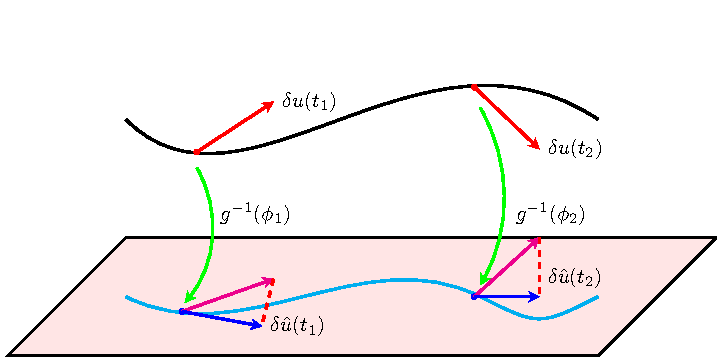
\includegraphics[width=0.4\textwidth]{jacobian_full_slice}
  \caption{slice}
  \label{fig:slice}
\end{figure}
The benefit of symmetry reduction is manifest.
The dimension of the symmetry reduced state space is one less than that
of the full state space. Also, the marginal \Fv\ corresponding to
the symmetry tangent direction disappears during the projection process.
Moreover, relative \po s are transformed to closed orbits in the slice.

Now, we turn to the shadowing process in the symmetry reduced state space.
we run a long integration of an ergodic trajectory,
and record the events where this orbit shadows a specific \po\ for at
least one period. For each point $\hat{u}(x, t)$
on the ergodic orbit during the shadowing period,
define its difference vector
\begin{equation}
  \label{eq:dif}
  \Delta \hat{u}(x,t) = \hat{u}(x, t) -\hat{u}_p(x_p, t_p)
  \,.
\end{equation}
Here $\hat{u}_p(x_p, t_p)$ is a point on the \po\ such that the norm
of $\Delta \hat{u}(x,t)$ is minimal when $\hat{u}_p(x_p, t_p)$
travels this \po. Basically, we can regard
$\hat{u}_p(x_p, t_p)$ as the point that attracts or repulses the ergodic
orbit at time $t$. Then $\Delta \hat{u}(x,t)$ is presumably
controlled by \Fv s at  $\hat{u}_p(x_p, t_p)$ at least when
$||\Delta \hat{u}(x,t)||$ is small enough.
If the asymptotic dynamics resides in a finite dimensional manifold,
then we expect that a subset of \Fv s could give a faithful
expansion of $\Delta \hat{u}$. More specifically,
$\Delta \hat{u}$ can be decomposed as
$\Delta \hat{u}(x, t) = v_k(x, t) + w_k(x,t)$.
Here, $v_k(x, t)$ is the part in the subspace spanned by the
leading $k$ \Fv s, and $w_k(x,t)$ is the part perpendicular to
such subspace. If the leading $k$ \Fv s generate a faithful
expansion of the \inm\ locally and assume the \inm\  has
a quadratic structure near \po s, then
$||w_k(x, t)|| \propto ||v_k(x,t)||^2$, otherwise,
$||w_k(x, t)||$ should decreases
slower than $||v_k(x,t)||^2$ as the ergodic orbit approaches the
\po. Denote the threshold of such $k$ as $k_c$.
Also denote  $\theta(x,t)$ the angle
between $v_k(x, t)$ and $\Delta \hat{u}(x, t)$. The analysis
above simply states that for $k \ge k_c$,
$\frac{\sin\theta}{||\Delta \hat{u}||} \propto \frac{1}{||w||+1}$,
which
is close to linear when $||\Delta \hat{u}||$ is small; while,
for $k \le k_c$,
$\frac{\sin\theta}{||\Delta \hat{u}||} > \frac{1}{||w||+1}$.
\begin{figure}[h]
  \centering
  \begin{minipage}{.23\textwidth}
    \centering \small{\texttt{(a)}}
    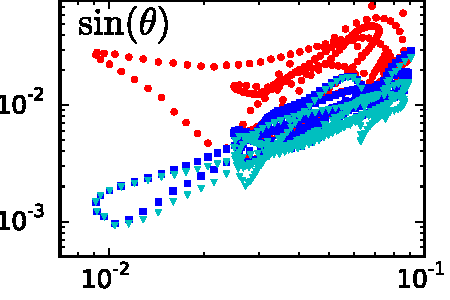
\includegraphics[width=\textwidth]{ppo4No6}
  \end{minipage}
  \begin{minipage}{.23\textwidth}
    \centering \small{\texttt{(b)}}
    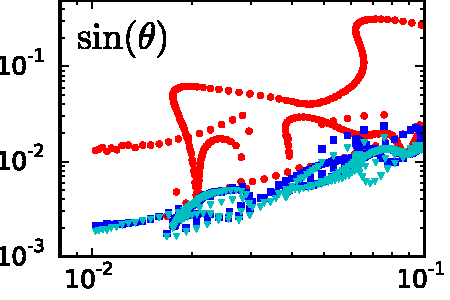
\includegraphics[width=\textwidth]{rpo4No1}
  \end{minipage}
  \begin{minipage}{.23\textwidth}
    \centering \small{\texttt{(c)}}
    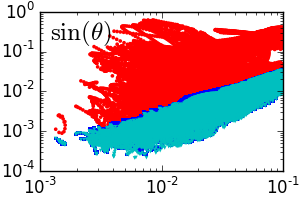
\includegraphics[width=\textwidth]{rpo4many}
  \end{minipage}
  \begin{minipage}{.23\textwidth}
    \centering \small{\texttt{(d)}}
    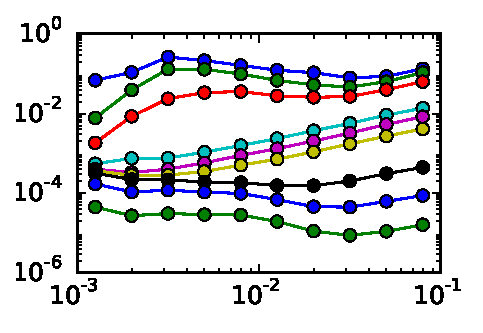
\includegraphics[width=\textwidth]{rpo4manyAverage}
  \end{minipage}
  \caption{
    (Color online) $sin(\theta)$ versus $||\Delta \hat{u}||$.
    (a) and (b) show one shadowing event of $\cycle{ppo}_{33.39}$
    and  $\cycle{rpo}_{34.64}$ respectively
    with  $k=6$ (red), $k=7$ (blue) and $k=8$ (green).
    (c) represents a total 217 shadowing events of
    $\cycle{rpo}_{34.64}$. (d) is the averaged form of (c) for
    $k=4, 5, 6, 7, 9, 11, 17, 21, 25$ from up to down.
  }
  \label{fig:shadow}
\end{figure}

\refFig{fig:shadow} shows our experimental result with
2 different orbits: $\cycle{ppo}_{33.39}$
and $\cycle{rpo}_{34.64}$. We see from panel (a) and (b) that
angles with $k=6$ departure from that with $k=7$ and is
almost one order larger; while angles with $k=7$ stay close
to that of $k=8$, which means that adding the $8$th \Fv\
only improve the expansion negligibly. This is not an accident
for this two shadowing events. As shown in panel (c), the
totality of 217 shadowing events of $\cycle{rpo}_{34.64}$
shows similar
behavior. Note the angle cloud of $k=7$ almost overlaps with that
of $k=8$. Panel (d) gives the histogram average of the angle
cloud in (c) but with a larger range of $k$ values. We see that
it is almost a straight line for $k=7$ except the twist close to
$||\Delta \hat{u}|| = 10^{-3}$, due to much fewer data points
at extremely close approach. We also notice that for larger
$k$, for example $k=17$, as the ergodic orbit approaches the \po, the
angle first decreases and then increases until saturates with that of
$k=7$. The reason is that when two orbits
are far away, the difference vector could almost be thought of as a
random vector, so larger $k$ gives better expansion. When these two
orbits gets closer, only the effective subset of \Fv s makes dominating
contribution to the expansion.

Therefore, the study of shadowing
in the symmetry reduced state space effectively tells us that
there is a minimal
subset of \Fv s which can effectively expand the \inm\ locally, and the
threshold number is 7. This confirms the result in the partial
hyperbolicity experiments since symmetry reduction reduces the dimension
of inertial manifold by one.

In conclusion, by studying the partial hyperbolic properties of the
tangent bundle via periodic
orbits and their associated \Fv s
and by investigating their shadowing events,
we obtained a lower bound on the
dimension of \inm\ in 1D \KSe. We exercise caution in our statement
since for large complex systems, several distinct strange attractors
may exist, and they probably have different topological structures.
The method we presented in this paper only gives a local
description of the geometry of \inm. Nonetheless, this lower bound
benefits people in determining how to truncate the original
infinite dimensional PDE into a finite set of ODEs for numerical
simulation. For example, as shown in\rf{foias88},
the 3-mode approximation
of the \inm\ of 1D \KSe\ fails to preserve the structure of its
bifurcation diagram.

Also, we choose to work in the symmetry reduced state space
because the dimensionality is reduced and it gives the
right picture of shadowing events between invariant tori.

The big challenge of this method is to first obtain
a set of periodic orbits and try to find shadowing
events, which is extremely hard for high dimensional systems.
Fortunately, research on this direction has made remarkable
progress in the last 20 years. We are optimistic to apply this
method to other more complicated spatiotemporal chaotic systems
in future.


\acknowledgements

We are indebted to
W. Hu,
Al Soyu
and
N. Ott Gain
for stimulating discussions,
and to
Mohammad M. Farazmand
for
a critical reading of the manuscript.
X.~D. and P.~C. were supported by
NSF~DMS-1211827.
P.~C.\ thanks the family of late G.~Robinson,~Jr.\ for continued support.

%==================================================
\bibliography{../../bibtex/siminos}

\ifboyscout
\newpage
\newcommand{\toCB}{\marginpar{\footnotesize 2CB}}  % to compare with ChaosBook
\newcommand{\inCB}{\marginpar{\footnotesize now in CB}} % entered in ChaosBook
Possible titles for this paper, \refref{DCTSCD14}:

``The physical dimension of a \KS\ flow.''

% \input ../blog/BudCvi14edits
\fi %end of internal draft switch

\section{Blog}
\label{sec:blog}

\begin{description}

\item[2015-9-20 Xiong] I am not convinced by the previous
statements that the dimension of inertial manifold for
\KSe\ at $L=22$ is exactly 8. I think this is only a lower bound.
I have a simple reasoning. The Kaplan-Yorke dimension\rf{KapYor79, FaOttYo83}
\beq
    D_{KY}= k + \frac{1}{|\Lyap^{(k+1)}|} \sum_{i=1}^k \Lyap^{(i)}
\,,
\ee{KapYorDim}
where $k$ is the largest integer such that the Lyapunov exponents sum
$\sum_{i=1}^k \Lyap^{(i)}>0$,
is formulated as the lower bound of the dimension of strange attractor.
For hyperbolic systems,  $D_{KY}$  could be larger than the number of
expanding \cLvs, so the dimension
of inertial manifold should be larger than the number of
expanding \cLvs, At the same time, since the angle
between expanding bundle and contracting bundle is bounded away from
zero, then our method will say that the dimension of the inertial
manifold is just the number of expanding directions. These two
statements are contradicting.

\item[2015-10-02 Xiong] I just find the explanation of the linear
relation in shadowing experiments is problematic.

\end{description}


\end{document}
